\documentclass[12pt]{scrartcl}

\usepackage[T1]{fontenc}
\usepackage[utf8]{inputenc}
\usepackage{amsmath}
\usepackage{amsfonts}
\usepackage{amssymb}
\usepackage{amsbsy}
\usepackage{graphicx}
\usepackage{float}
\usepackage{array}
\usepackage{booktabs}
\usepackage{multirow}
\usepackage{bm}
\usepackage{verbatim}
\usepackage[english]{babel}
\usepackage{color}
\usepackage{url}
\usepackage{fancybox}
\usepackage[stable]{footmisc}
\usepackage[format=plain,labelfont=bf]{caption}
\usepackage{fancyhdr}
\usepackage{natbib}
\usepackage{calc}
\usepackage{textcomp}
\usepackage[pdftex,pdfborder={0 0 0}]{hyperref}
\usepackage{pdfpages}
\usepackage{tikz}
\usetikzlibrary{shapes,arrows,decorations.pathmorphing}

\renewcommand*{\familydefault}{\sfdefault}

% Margins
\addtolength{\textheight}{1.0cm}
\addtolength{\oddsidemargin}{-0.5cm}
\addtolength{\evensidemargin}{-0.5cm}
\addtolength{\textwidth}{1.0cm}
\parindent=0em

% New math commands
\newcommand{\overbar}[1]{\mkern 1.5mu\overline{\mkern-1.5mu#1\mkern-1.5mu}\mkern 1.5mu}
\DeclareMathOperator{\diag}{diag}
\DeclareMathOperator{\Diag}{Diag}
\DeclareMathOperator{\tr}{tr}
\DeclareMathOperator{\Cov}{Cov}
\DeclareMathOperator{\Cor}{Cor}
\newcommand\independent{\protect\mathpalette{\protect\independenT}{\perp}}
\def\independenT#1#2{\mathrel{\setbox0\hbox{$#1#2$}%
\copy0\kern-\wd0\mkern4mu\box0}}

% Appropriate font for \mathcal{}
\DeclareSymbolFont{cmmathcal}{OMS}{cmsy}{m}{n}
\DeclareSymbolFontAlphabet{\mathcal}{cmmathcal}

% Set subscript and superscripts positions
\everymath{
\fontdimen13\textfont2=5pt
\fontdimen14\textfont2=5pt
\fontdimen15\textfont2=5pt
\fontdimen16\textfont2=5pt
\fontdimen17\textfont2=5pt
}

% Bibliography style
\setlength{\bibsep}{1pt}

% Part
\renewcommand\partheadstartvskip{\clearpage\null\vfil}
\renewcommand\partheadmidvskip{\par\nobreak\vskip 20pt\thispagestyle{empty}}
\renewcommand\partheadendvskip{\vfil\clearpage}
\renewcommand\raggedpart{\centering}

\begin{document}
\title{Multivariate localization}
\author{Benjamin Ménétrier}
\date{Last update: \today}

\thispagestyle{empty}

\maketitle
\begin{center}
Documentation for the code "BUMP", distributed under the CeCILL-C license.\\
Copyright \copyright 2015-... UCAR, CERFACS, METEO-FRANCE and IRIT
\end{center}

\tableofcontents

\clearpage


\section{Framework}
A localization matrix $\mathbf{L} \in \mathbb{R}^{n \times n}$ is applied to a multivariate state vector $\mathbf{x} \in \mathbb{R}^n$, built as the concatenation of $p$ sub-vectors:
\begin{align}
\mathbf{x} = \left( \begin{array}{c}
\mathbf{x}_1 \\[1ex]
\hline
\vdots \\
\hline
\mathbf{x}_p
\end{array} \right)
\end{align}
where $\mathbf{x}_i$ is the sub-vector for variable $i$, of size $n_i$. Obviously, $\displaystyle n = \sum_{i=1}^p n_i$.\\
$  $\\
The localization matrix is split into blocks:
\begin{align*}
\mathbf{L} = \left( \begin{array}{ccc}
\mathbf{L}_{11} & \cdots & \mathbf{L}_{1p} \\
\vdots & \ddots & \vdots \\
\mathbf{L}_{p1} & \cdots & \mathbf{L}_{pp}
\end{array} \right)
\end{align*}
The problem is to design a positive semi-definite localization matrix:
\begin{itemize}
\item $\mathbf{L}_{ii}$ should be positive semi-definite,
\item the constraint on $\mathbf{L}_{ij}$ for $i \ne j$ is less obvious...
\end{itemize}
The solution is to build a square-root $\mathbf{U} \in \mathbb{R}^{n \times m}$ of the localization matrix $\mathbf{L}$, such that $\mathbf{L} = \mathbf{UU}^\textrm{T}$. The control vector $\mathbf{v}$ such that $\mathbf{x} = \mathbf{U} \mathbf{v}$ is defined in the control space of size $m$.\\

\section{Univariate specific blocks}
The simplest method is to design $\mathbf{U}$ as:
\begin{align}
\mathbf{U} = \left( \begin{array}{cccc}
\mathbf{U}_1 & 0 & \cdots & 0 \\
0 & \mathbf{U}_2 & \cdots & 0 \\
\vdots & \vdots & \ddots & \vdots \\
0 & 0 & \cdots & \mathbf{U}_p
\end{array} \right)
\end{align}
where $\mathbf{U}_i \in \mathbb{R}^{n_i \times m_i}$, $m_i$ being the size of the control sub-vector related to variable $i$ with $\displaystyle m = \sum_{i=1}^p m_i$. The resulting localization matrix is:
\begin{align}
\mathbf{L} = \mathbf{U} \mathbf{U}^\mathrm{T} = \left( \begin{array}{cccc}
\mathbf{U}_1 \mathbf{U}_1^\mathrm{T} & 0 & \cdots & 0 \\
0 & \mathbf{U}_2 \mathbf{U}_2^\mathrm{T} & \cdots & 0 \\
\vdots & \vdots & \ddots & \vdots \\
0 & 0 & \cdots & \mathbf{U}_p \mathbf{U}_p^\mathrm{T}
\end{array} \right)
\end{align}
In this case, auto-localization blocks are well defined:
\begin{align}
\mathbf{L}_{ii} = \mathbf{U}_i \mathbf{U}_i^\mathrm{T}
\end{align}
but cross-localization blocks $\mathbf{L}_{ij}$ for $i \ne j$ are zero.\\
$  $\\
\textbf{Advantages:} well-adapted for large differences between variables length-scales and/or for small cross-correlation (sampling noise is canceled).\\
\textbf{Drawbacks:} ill-adapted for significant cross-correlations (signal is lost).\\
\textbf{Cost:} $p$ applications of $\mathbf{U}_i$.

\section{Multivariate specific blocks}

\subsection{State grid interpolation}
A second method is to perform interpolations to and from a common state grid of size $\overbar{n}$. $\mathbf{S}^\mathrm{s}_i \in \mathbb{R}^{n_i \times \overbar{n}}$ is defined as the interpolation from the common state grid to the state grid of variable $i$. We gather these matrices into a global state interpolation matrix $\mathbf{S}^\mathrm{s}$:
\begin{align}
\mathbf{S}^\mathrm{s} = \left( \begin{array}{cccc}
\mathbf{S}^\mathrm{s}_1 & 0 & \cdots & 0 \\
0 & \mathbf{S}^\mathrm{s}_2 & \cdots & 0 \\
\vdots & \vdots & \ddots & \vdots \\
0 & 0 & \cdots & \mathbf{S}^\mathrm{s}_p
\end{array} \right)
\end{align}
A specific block $\overbar{\mathbf{U}}_i \in \mathbb{R}^{\overbar{n} \times m}$ is applied to each variable $i$:
\begin{align}
\mathbf{U} = \mathbf{S}^\mathrm{s} \left( \begin{array}{c}
\overbar{\mathbf{U}}_1 \\
\vdots \\
\overbar{\mathbf{U}}_p
\end{array} \right)
\end{align}
The resulting localization matrix is:
\begin{align}
\mathbf{L} = \mathbf{U} \mathbf{U}^\mathrm{T} = \mathbf{S}^\mathrm{s} \left( \begin{array}{ccc}
\overbar{\mathbf{U}}_1 \overbar{\mathbf{U}}_1^\mathrm{T} & \cdots & \overbar{\mathbf{U}}_1 \overbar{\mathbf{U}}_p^\mathrm{T} \\
\vdots & \ddots & \vdots  \\
\overbar{\mathbf{U}}_p \overbar{\mathbf{U}}_1^\mathrm{T} & \cdots & \overbar{\mathbf{U}}_p \overbar{\mathbf{U}}_p^\mathrm{T}
\end{array} \right) \mathbf{S}^{\mathrm{s} \mathrm{T}}
\end{align}
In this case, each auto- or cross-localization block is given by:
\begin{align}
\mathbf{L}_{ij} = \mathbf{S}^\mathrm{s}_i \overbar{\mathbf{U}}_i \overbar{\mathbf{U}}_j^\mathrm{T} \mathbf{S}_j^{\mathrm{s} \mathrm{T}}
\end{align}

\subsection{Control grid interpolation}
An alternative to this method is to perform interpolations to and from a common control grid of size $\overbar{m}$. $\mathbf{S}^\mathrm{c}_i \in \mathbb{R}^{m_i \times \overbar{m}}$ is defined as the interpolation from the common vector grid to the control grid of variable $i$. We can write a global interpolation matrix $\mathbf{S}^\mathrm{c}$ as:
\begin{align}
\mathbf{S}^\mathrm{c} = \left( \begin{array}{cccc}
\mathbf{S}^\mathrm{c}_1 & 0 & \cdots & 0 \\
0 & \mathbf{S}^\mathrm{c}_2 & \cdots & 0 \\
\vdots & \vdots & \ddots & \vdots \\
0 & 0 & \cdots & \mathbf{S}^\mathrm{c}_p
\end{array} \right)
\end{align}
A specific block $\mathbf{U}_i \in \mathbb{R}^{n_i \times m_i}$ is applied to each variable:
\begin{align}
\mathbf{U} = \left( \begin{array}{c}
\mathbf{U}_1 \\
\vdots \\
\mathbf{U}_p
\end{array} \right) \mathbf{S}^\mathrm{c}
\end{align}
The resulting localization matrix is $\mathbf{L} = \mathbf{U} \mathbf{U}^\mathrm{T}$ with each auto- or cross-localization block given by:
\begin{align}
\mathbf{L}_{ij} = \mathbf{U}_i \mathbf{S}^\mathrm{c}_i \mathbf{S}_j^{\mathrm{c} \mathrm{T}} \mathbf{U}_j^\mathrm{T}
\end{align}

\subsection{Interpolation error}
We assume that every interpolation $\mathbf{S}^\mathrm{s}$ or $\mathbf{S}^\mathrm{c}$ can be expanded as $\mathbf{S} = \mathbf{T} + \mathbf{E}$ where $\mathbf{T}$ is the "true" interpolation, i.e. the best we can get with a linear operator, and $\mathbf{E} = \mathbf{S} - \mathbf{T}$ the resulting error.
Thus:
\begin{itemize}
\item For the state grid interpolation with specific blocks:
\begin{align}
\mathbf{L}_{ij} & = \mathbf{S}^\mathrm{s}_i \overbar{\mathbf{U}}_i \overbar{\mathbf{U}}_j^\mathrm{T} \mathbf{S}_j^{\mathrm{s} \mathrm{T}} \nonumber \\
& = \mathbf{T}^\mathrm{s}_i \overbar{\mathbf{U}}_i \overbar{\mathbf{U}}_j^\mathrm{T} \mathbf{T}_j^{\mathrm{s} \mathrm{T}} + \mathbf{E}^\mathrm{s}_i \overbar{\mathbf{U}}_i \overbar{\mathbf{U}}_j^\mathrm{T} \mathbf{T}_j^{\mathrm{s} \mathrm{T}} + \mathbf{T}^\mathrm{s}_i \overbar{\mathbf{U}}_i \overbar{\mathbf{U}}_j^\mathrm{T} \mathbf{E}_j^{\mathrm{s} \mathrm{T}} + \mathbf{E}^\mathrm{s}_i \overbar{\mathbf{U}}_i \overbar{\mathbf{U}}_j^\mathrm{T} \mathbf{E}_j^{\mathrm{s} \mathrm{T}}
\end{align}
and similarly for the state grid interpolation with a common block.
\item For the control grid interpolation:
\begin{align}
\mathbf{L}_{ij} & = \mathbf{U}_i \mathbf{S}^\mathrm{c}_i \mathbf{S}_j^{\mathrm{c} \mathrm{T}} \mathbf{U}_j^\mathrm{T} \nonumber \\
& = \mathbf{U}_i \mathbf{T}^\mathrm{c}_i \mathbf{T}_j^{\mathrm{c} \mathrm{T}} \mathbf{U}_j^\mathrm{T} + \mathbf{U}_i \mathbf{E}^\mathrm{c}_i \mathbf{T}_j^{\mathrm{c} \mathrm{T}} \mathbf{U}_j^\mathrm{T} + \mathbf{U}_i \mathbf{T}^\mathrm{c}_i \mathbf{E}_j^{\mathrm{c} \mathrm{T}} \mathbf{U}_j^\mathrm{T} + \mathbf{U}_i \mathbf{E}^\mathrm{c}_i \mathbf{E}_j^{\mathrm{c} \mathrm{T}} \mathbf{U}_j^\mathrm{T}
\end{align}
\end{itemize}
Assuming that interpolation errors are random with a short correlation length-scale, the control grid interpolation looks like a better option since a smoothing is always applied as the last operator. However, even with the state grid interpolation:
\begin{itemize}
\item either the interpolation error is smoothed in subsequent operators,
\item or the interpolation error is itself applied on smoothed fields at high-resolution, leading to small interpolation errors.
\end{itemize}
As a conclusion, we don't think that interpolation error is a major issue that should favor one approach or the other.

\subsection{Localization amplitude}
We denote $\overbar{\mathbf{u}}$ the k$^\textrm{th}$ column of $\overbar{\mathbf{U}}_i$ and $\overbar{\mathbf{u}}'$ the k$^\textrm{th}$ column of $\overbar{\mathbf{U}}_j$. The k$^\textrm{th}$ diagonal coefficient of $\overbar{\mathbf{U}}_i \overbar{\mathbf{U}}_j^\mathrm{T}$ is given by $\langle \overbar{\mathbf{u}},\overbar{\mathbf{u}}' \rangle$, where $\langle \cdot, \cdot \rangle$ denotes the canonical inner product. The Cauchy-Schwartz inequality imposes that:
\begin{align}
\vert \langle \overbar{\mathbf{u}},\overbar{\mathbf{u}}' \rangle \vert & \le \sqrt{\langle \overbar{\mathbf{u}},\overbar{\mathbf{u}} \rangle \langle \overbar{\mathbf{u}}',\mathbf{u}' \rangle}
\end{align}
Thus, the cross-localization amplitude between variables $i$ and $j$ is necessarily smaller than the geometric mean of the auto-localization amplitudes for variables $i$ and $j$. Besides, the more the vectors $\overbar{\mathbf{u}}$ and $\overbar{\mathbf{u}}'$ have different shapes, the smaller their inner product and the smaller the cross-localization amplitude.
\begin{center}
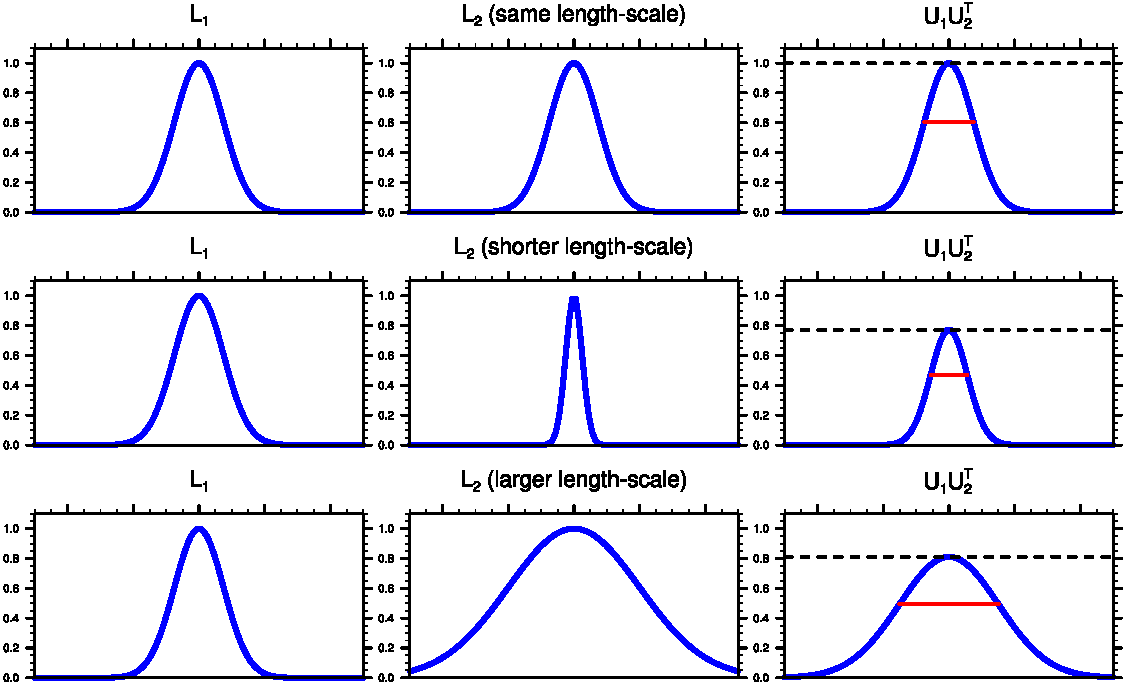
\includegraphics[width=\linewidth]{convolution_exp.pdf}
\captionof{figure}{1D illustration of the product of two localization square-root, with Gaussian localization functions. The dashed black line shows the function amplitude, while the solid red line shows the function length-scale.}
\end{center}
$  $\\
\textbf{Advantages:} well-adapted for large differences between variables length-scales.\\
\textbf{Drawbacks:} no control on the cross-localization amplitude.\\
\textbf{Cost:} $p$ applications of $\overbar{\mathbf{U}}_i$.

\section{Common block}

\subsection{Basic method}
A third method is to apply a common block $\overbar{\mathbf{U}} \in \mathbb{R}^{\overbar{n} \times m}$ to all variables, with a state grid interpolation:
\begin{align}
\mathbf{U} = \mathbf{S}^\mathrm{s} \left( \begin{array}{c}
\overbar{\mathbf{U}} \\
\vdots \\
\overbar{\mathbf{U}}
\end{array} \right) = \mathbf{S}^\mathrm{s} \left( \begin{array}{c}
\mathbf{I}_{\overbar{n}} \\
\vdots \\
\mathbf{I}_{\overbar{n}} \\
\end{array} \right) \overbar{\mathbf{U}}
\end{align}
where $\mathbf{I}_{\overbar{n}} \in \mathbb{R}^{\overbar{n} \times \overbar{n}}$ is the identity matrix. It should be noted that to apply $\mathbf{U}$, the matrix $\overbar{\mathbf{U}}$ needs to be applied only once. The resulting localization matrix is:
\begin{align}
\mathbf{L} = \mathbf{U} \mathbf{U}^\mathrm{T} = \mathbf{S}^\mathrm{s} \left( \begin{array}{ccc}
\overbar{\mathbf{U}} \overbar{\mathbf{U}}^\mathrm{T} & \cdots & \overbar{\mathbf{U}} \overbar{\mathbf{U}}^\mathrm{T} \\
\vdots & \ddots & \vdots  \\
\overbar{\mathbf{U}} \overbar{\mathbf{U}}^\mathrm{T} & \cdots & \overbar{\mathbf{U}} \overbar{\mathbf{U}}^\mathrm{T}
\end{array} \right) \mathbf{S}^{\mathrm{s} \mathrm{T}}
\end{align}
In this case, each auto- or cross-localization block is given by:
\begin{align}
\mathbf{L}_{ij} = \mathbf{S}^\mathrm{s}_i \overbar{\mathbf{U}} \overbar{\mathbf{U}}^\mathrm{T} \mathbf{S}_j^{\mathrm{s} \mathrm{T}}
\end{align}
It should be noted that this approach is inconsistent with the optimal linear filtering theory. Indeed, the cross-correlation between different variables, even at zero separation, is lower than 1 (i.e. the value for auto-correlations). Thus, the cross-localization should be lower than the auto-localization at zero separation, whereas $\left[\overbar{\mathbf{U}} \overbar{\mathbf{U}}^\mathrm{T}\right]_{ii}$ is applied in both case.\\
$  $\\
\textbf{Advantages:} lower cost.\\
\textbf{Drawbacks:} ill-adapted for large differences between variables length-scales and/or for small cross-correlations (sampling noise is kept).\\
\textbf{Cost:} one application of $\overbar{\mathbf{U}}$.

\subsection{Weighted variant}
A fourth method is to apply a lower triangular square-root of weighted common blocks $\overbar{\mathbf{U}} \in \mathbb{R}^{\overbar{n} \times m}$, with a state grid interpolation:
\begin{align}
\mathbf{U} & = \mathbf{S}^\mathrm{s} \left( \begin{array}{cccc}
Q_{1,1} \overbar{\mathbf{U}} & 0 & \cdots & 0 \\
Q_{2,1} \overbar{\mathbf{U}} & Q_{2,2} \overbar{\mathbf{U}} & \ddots & \vdots \\
\vdots & \ddots & \ddots & 0 \\
Q_{p,1} \overbar{\mathbf{U}} & \cdots & Q_{p,p-1} \overbar{\mathbf{U}} & Q_{p,p} \overbar{\mathbf{U}}
\end{array} \right) \\
 & = \mathbf{S}^\mathrm{s} \left( \begin{array}{cccc}
Q_{1,1} \mathbf{I}_{\overbar{n}} & 0 & \cdots & 0 \\
Q_{2,1} \mathbf{I}_{\overbar{n}} & Q_{2,2} \mathbf{I}_{\overbar{n}} & \ddots & \vdots \\
\vdots & \ddots & \ddots & 0 \\
Q_{p,1} \mathbf{I}_{\overbar{n}} & \cdots & Q_{p,p-1} \mathbf{I}_{\overbar{n}} & Q_{p,p} \mathbf{I}_{\overbar{n}}
\end{array} \right) \left( \begin{array}{cccc}
\overbar{\mathbf{U}} & 0 & \cdots & 0 \\
0 & \overbar{\mathbf{U}} & \ddots & \vdots \\
\vdots & \ddots & \ddots & 0 \\
0 & \cdots & 0 & \overbar{\mathbf{U}}
\end{array} \right)
\end{align}
where $\mathbf{I}_{\overbar{n}} \in \mathbb{R}^{\overbar{n} \times \overbar{n}}$ is the identity matrix. It should be noted that to apply $\mathbf{U}$, the matrix $\overbar{\mathbf{U}}$ needs to be applied $p$ times. The resulting localization matrix is:
\begin{align}
\mathbf{L} = \mathbf{U} \mathbf{U}^\mathrm{T} = \mathbf{S}^\mathrm{s} \left( \begin{array}{ccc}
W_{1,1} \overbar{\mathbf{U}} \overbar{\mathbf{U}}^\mathrm{T} & \cdots & W_{1,p} \overbar{\mathbf{U}} \overbar{\mathbf{U}}^\mathrm{T} \\
\vdots & \ddots & \vdots  \\
W_{p,1} \overbar{\mathbf{U}} \overbar{\mathbf{U}}^\mathrm{T} & \cdots & W_{p,p} \overbar{\mathbf{U}} \overbar{\mathbf{U}}^\mathrm{T}
\end{array} \right) \mathbf{S}^{\mathrm{s} \mathrm{T}}
\end{align}
where $\mathbf{W} = \mathbf{Q} \mathbf{Q}^\textrm{T}$. In this case, each auto- or cross-localization block is given by:
\begin{align}
\mathbf{L}_{ij} = W_{i,j} \mathbf{S}^\mathrm{s}_i \overbar{\mathbf{U}} \overbar{\mathbf{U}}^\mathrm{T} \mathbf{S}_j^{\mathrm{s} \mathrm{T}}
\end{align}
The actual process would be reversed: first define $\mathbf{W}$, and its square-root decomposition $\mathbf{Q}$. Since $\mathbf{W}$ and $\mathbf{Q}$ are square matrices of size $p$, a Cholesky decomposition can work.\\
$  $\\
\textbf{Advantages:} precise control on the cross-localization amplitude.\\
\textbf{Drawbacks:} ill-adapted for large differences between variables length-scales.\\
\textbf{Cost:} $p$ applications of $\overbar{\mathbf{U}}$.

\section{Applications}
The approaches above can be used to localize 3D variables located on different points of the grid (e.g. Arakawa C grid).\\
$  $\\
It can also work to maintain a non-zero cross-localization between 3D and 2D variables, which is needed if they are correlated. The usual practice is to build an extended 3D grid with one more level at the bottom, and to copy the 2D variable on this extra level. The formalism described above can be used to understand this approach: the state grid interpolation is a simple copy of the 2D variable on the extra level, and a copy of the 3D variable on the remaining levels above.\\
$  $\\
Using a common block $\overbar{\mathbf{U}}$ can lead to some issues when the 3D and 2D variables have very different length-scales (e.g. temperature and surface pressure). However, we can also use the state grid interpolation with two specific blocks $\overbar{\mathbf{U}}_{3D}$ and $\overbar{\mathbf{U}}_{2D}$, which are both defined on the extended grid.\\
$  $\\
The control grid interpolation approach is not suitable to cross-localize 3D and 2D variables, since it is not possible to define cross-localizations on their specific grids.

\clearpage

\bibliographystyle{mybib-en}
\bibliography{multivariate_localization}
\end{document}
